%http://www.daniel-brettschneider.de/allgemein/latex-vorlage-fur-hausarbeiten-oder-abschlussarbeiten
\documentclass[12pt,a4paper,bibliography=totocnumbered,listof=totocnumbered, abstracton]{scrartcl}

\usepackage[autostyle=true,german=quotes]{csquotes}
\usepackage[utf8]{inputenc}
\usepackage{amsmath}
\usepackage{amsfonts}
\usepackage{amssymb}
\usepackage{amsthm}
\usepackage{graphicx}
\usepackage{fancyhdr}
\usepackage{tabularx}
\usepackage{geometry}
\usepackage{setspace}
\usepackage[right]{eurosym}
\usepackage[printonlyused]{acronym}
\usepackage{subfig}
\usepackage{floatflt}
\usepackage[usenames,dvipsnames]{color}
\usepackage{colortbl}
\usepackage{paralist}
\usepackage{array}
\usepackage{titlesec}
\usepackage{parskip}
\usepackage[right]{eurosym}
\usepackage[subfigure,titles]{tocloft}
\usepackage[pdfpagelabels=true]{hyperref}
\usepackage[ngerman]{babel}
\usepackage{booktabs}
\usepackage{listings}
\usepackage{csquotes}
\usepackage{siunitx}
\newtheoremstyle{Umgebung}	% name
{20pt}	% Space above, empty = `usual value'
{20pt} % Space below
{} % Body font
{} % Indent amount (empty = no indent, \parindent = para indent)
{\bfseries} % Thm head font
{} % Punctuation after thm head
{\newline} % Space after thm head: \newline = linebreak
{} % Thm head spec


\theoremstyle{Umgebung}

\lstset{basicstyle=\footnotesize, captionpos=b, breaklines=true, showstringspaces=false, tabsize=2, frame=lines, numbers=left, numberstyle=\tiny, xleftmargin=2em, framexleftmargin=2em}
\makeatletter
\def\l@lstlisting#1#2{\@dottedtocline{1}{0em}{1em}{\hspace{1,5em} Lst. #1}{#2}}
\makeatother
\geometry{a4paper, top=27mm, left=30mm, right=20mm, bottom=35mm, headsep=10mm, footskip=12mm}
\hypersetup{unicode=false, pdftoolbar=true, pdfmenubar=true, pdffitwindow=false, pdfstartview={FitH},
	pdftitle={Ausarbeitung Fuzzy-Reglung},
	pdfauthor={Joel Bartelheimer, Nico Müller},
	pdfsubject={Ausarbeitung Fuzzy-Reglung},
	pdfcreator={\LaTeX\ with package \flqq hyperref\frqq},
	pdfproducer={pdfTeX \the\pdftexversion.\pdftexrevision},
	pdfkeywords={Ausarbeitung Fuzzy-Regler},
	pdfnewwindow=true,
	colorlinks=true,linkcolor=black,citecolor=black,filecolor=magenta,urlcolor=black}
\pdfinfo{/CreationDate (D:20110620133321)}
\begin{document}
\titlespacing{\section}{0pt}{12pt plus 4pt minus 2pt}{-6pt plus 2pt minus 2pt}
% Kopf- und Fusszeile
\renewcommand{\sectionmark}[1]{\markright{#1}}
\renewcommand{\leftmark}{\rightmark}
\pagestyle{fancy}
\lhead{}
\chead{}
\rhead{\thesection\space\contentsname}
\lfoot{Ausarbeitung Fuzzy-Reglung}
\cfoot{}
\rfoot{ Seite \thepage}
\renewcommand{\headrulewidth}{0.4pt}
\renewcommand{\footrulewidth}{0.4pt}
% Vorspann
\renewcommand{\thesection}{\Roman{section}}
\renewcommand{\theHsection}{\Roman{section}}
\pagenumbering{roman}
% ----------------------------------------------------------------------------------------------------------
% Titelseite
% ----------------------------------------------------------------------------------------------------------
\thispagestyle{empty}
\begin{center}
	
\includegraphics[width=5cm]{img/thm2.png}\\
	\vspace*{2cm}
	\Large
	\textbf{Fachbereich}\\
	\textbf{Mathematik, Naturwissenschaften und Informatik }\\
	\vspace*{2cm}
			\Huge
	\textbf{Fuzzy-Regelung Ausarbeitung}\\
	\vspace*{1.5cm}
		\small
		\textbf{Im Rahmen der Veranstaltung:}\\
		\Large
	\textbf{Praktikum Künstliche Intelligenz(CS5330)}\\
	\vspace*{2cm}
	

	\normalsize
	\newcolumntype{x}[1]{>{\raggedleft\arraybackslash\hspace{0pt}}p{#1}}
	\begin{tabular}{x{7.5cm}x{7.5cm}}
		\rule{0mm}{5ex}\textbf{Autoren:} 
		\newline 
		\newline Joel Bartelheimer
		\newline joel.bartelheimer@mni.thm.de
		\newline 
		\newline Nico Müller
		\newline nico.mueller@mni.thm.de
		\newline
		& 
		\rule{0mm}{5ex}\textbf{Eingereicht bei:} 
		\newline
		\newline  Prof. Dr. Wolfgang Henrich
		\newline
		\newline\rule{0mm}{5ex}\textbf{Abgabedatum:} 
		\newline 14.02.2017
		\newline
	\end{tabular} 
\end{center}
\pagebreak

% ----------------------------------------------------------------------------------------------------------
% Verzeichnisse
% ----------------------------------------------------------------------------------------------------------
% TODO Typ vor Nummer
\renewcommand{\cfttabpresnum}{Tab. }
\renewcommand{\cftfigpresnum}{Abb. }
\settowidth{\cfttabnumwidth}{Abb. 10\quad}
\settowidth{\cftfignumwidth}{Abb. 10\quad}
\titlespacing{\section}{0pt}{12pt plus 4pt minus 2pt}{2pt plus 2pt minus 2pt}
\singlespacing
\rhead{INHALTSVERZEICHNIS}
\renewcommand{\contentsname}{II Inhaltsverzeichnis}
\phantomsection
\addcontentsline{toc}{section}{\texorpdfstring{II \hspace{0.35em}Inhaltsverzeichnis}{Inhaltsverzeichnis}}
\addtocounter{section}{1}
\tableofcontents
\pagebreak
\rhead{VERZEICHNISSE}
\listoffigures
\pagebreak

% ----------------------------------------------------------------------------------------------------------
% Inhalt
% ----------------------------------------------------------------------------------------------------------
% Abstände Überschrift
\titlespacing{\section}{0pt}{12pt plus 4pt minus 2pt}{-6pt plus 2pt minus 2pt}
\titlespacing{\subsection}{0pt}{12pt plus 4pt minus 2pt}{-6pt plus 2pt minus 2pt}
\titlespacing{\subsubsection}{0pt}{12pt plus 4pt minus 2pt}{-6pt plus 2pt minus 2pt}
% Kopfzeile
\renewcommand{\sectionmark}[1]{\markright{#1}}
\renewcommand{\subsectionmark}[1]{}
\renewcommand{\subsubsectionmark}[1]{}
\lhead{Kapitel \thesection}
\rhead{\rightmark}
\onehalfspacing
\renewcommand{\thesection}{\arabic{section}}
\renewcommand{\theHsection}{\arabic{section}}
\setcounter{section}{0}
\pagenumbering{arabic}
\setcounter{page}{1}

\newtheorem{bsp}{Beispiel}
\newtheorem{defnt}{Definition}

% ----------------------------------------------------------------------------------------------------------
% Einleitung
% ----------------------------------------------------------------------------------------------------------

\begin{abstract} 
Die vorliegende Hausarbeit gibt einen Einstieg in die theoretische Fuzzy-Logik und behandelt dabei Fuzzy-Mengen, Fuzzy-Relation sowie Fuzzy-Operationen. Dem Leser soll bewusst gemacht werden worin sich die scharfe Mengenlehre von der der Fuzzy-Mengenlehre unterscheidet. An anschaulichen Beispielen wird erklärt was Linguistische Terme sind und wie diese repräsentiert werden können. Eigentliches Ziel ist die Untersuchung des Einsatzgebiets der Fuzzy-Regler, welches ein Teilgebiet der Fuzzy-Logik darstellt. Hier werden die Komponenten wie z.B. die Wissensbasis, das Fuzzyfizierungs- und Defuzzyfizierungs-Interface sowie die Entscheidungslogik vorgestellt. Da zur Zeit zwei Varianten (Mamdani sowie Takagi/Sugeno)  der Fuzzy-Regler verbreitet sind, werden diese beiden nacheinander vorgestellt und deren Vorteile aufgezeigt. Zuletzt werden die üblichen Defuzzifizierungsmethoden erklärt und an einem Beispiel veranschaulicht.
\end{abstract} 
\newpage

\section{Einleitung}

Um den Sinn sowie die Einsatzgebiete von Fuzzy-Logik zu verstehen, betrachten wir ein kurzes Beispiel: Ziel soll es sein einen Roboter zu bauen der Eier kochen kann. Wichtig hierbei ist, dass das Eigelb wachsweich sein sollte. Um den Vorgang des \enquote{Eierkochens} besser zu verstehen fragen wir bei einem Koch nach dem Perfekten Algorithmus nach. Er sagt uns: \enquote{werfe das Ei in kochendes Wasser und nehme es nach 5 Minuten wieder heraus}. Der Roboter arbeitet nun nach genau diesem Algorithmus, doch mussten wir feststellen, dass es vorkommen kann das manche Eier zu hart oder auch zu weich gekocht werden. Darauf hin sprechen wir erneut mit dem Koch. Diesmal sagt er uns, dass die Eier etwas länger kochen sollen falls sie größer sind und etwas kürzer kochen sollen wenn sie kleiner sind. Diese zwei Aussagen lassen sich nun schwer in einen Algorithmus umsetzen, da der Roboter nicht genau weiß was er unter einem kleiner bzw. größerem Ei verstehen soll. Er kann auch den Begriff \enquote{Etwas kürzer/länger} nicht begreifen. Um dem Roboter ein wenig zu helfen, definieren wir dass ein kleines Ei $40-49g$, ein normales Ei $50-60g$ und ein großes Ei $61-70g$ wiegt und das \enquote{Etwas kürzer/länger} eine Minute weniger- bzw. mehr bedeutet. Diesen Vorgang nennt man Partitionierung. Unser Roboter kann mit diesen Informationen die Eier schon fast annehmbar gut kochen. Wir vermuten jedoch, dass das System noch besser arbeiten könnte. Wenn ein Ei genau $60.99g$ wiegt, wird es von unserem Roboter für ein normales Ei gehalten und es wird genau 5 Minuten gekocht. Wäre es möglich, dass der menschliche Koch dieses Ei anders behandeln würde? Ja, er würde das Ei wahrscheinlich als ein mittelgroßes Ei behandeln und es 5.5 Minuten kochen, da es in der Gewichtseinstufung genau zwischen zwei Klassen liegt. Wie man ein solches Verhalten auf einen Roboter übertragen kann wird in den folgenden Kapiteln betrachtet.

\subsection{Anwendungsgebiete}

Fuzzy-Logik wurde schon erstmal 1964 in einen Artikel von Zadeh vorgestellt \cite{zadeh1965fuzzy}. In den 80er Jahren wurde dann Fuzzy-Logik vermehrt in Japan eingesetzt. Erfolgsgeschichten sind hierbei die U-Bahn in Sendai, und später die U-Bahn in Tokyo, die mit Hilfe von Fuzzy-Regelung eine sehr komfortables Anfahren und Abbremsen ermöglichen und effizienter arbeiten als ein menschlicher Bahnführer. Heute wird Fuzzy-Logik in Bildstabilisatoren für Kameras, Waschmaschinen oder der Automobil Industrie eingesetzt.

\section{Fuzzy-Logik Grundlagen}

Obwohl diese Ausarbeitung sich auf Fuzzy-Regelung spezialisiert, ist es notwendig die Grundbegriffe der Fuzzy-Logik zu verstehen. Die theoretischen Konzepte von Fuzzy-Mengen, Fuzzy-Relationen sowie Fuzzy-Operationen werden in diesem Kapitel wiederholt.

\subsection{Fuzzy-Logik Allgemein}

In der klassischen Mengenlehre, in der Domaine von Fuzzy-Logik auch scharfe Logik genannt, hat ein jedes Element $x_i$ eine eindeutige Zugehörigkeit zu einer Menge $X$. Dies bedeutet das jedes Element $x_i$ den Zugehörigkeitsgrad $\mu$ von genau $1$ oder $0$ hat. Diese strikte Klassifizierung ist im menschlichen Verständnis nicht intuitiv ausgeprägt. Einem Menschen fällt es einfacher eine wage Aussage wie z.B. \enquote{in etwa}, \enquote{relativ groß} o.Ä. zu treffen. Mithilfe der Fuzzy-Logik, in der Domaine von Fuzzy-Logik auch unscharfe Logik genannt, wird der strikte Zugehörigkeitsgrad aufgelöst, sodass jedes Element auch nur zum Teil einer Fuzzy-Menge angehören kann (siehe Abschnitte \ref{subsection:Fuzzy-Mengen}).

\label{subsection:Fuzzy-Mengen}
\subsection{Fuzzy-Mengen}

In der Domain der Fuzzy-Logik wird eine Menge über die Zugehörigkeitsgrade ihrer Elemente definiert. Die Zugehörigkeit eines Elementes $x$ zu einer Menge $A$ wird über die Zugehörigkeitsfunktion $\mu_A(x)$ definiert. Wichtig ist hierbei, dass jedes Element aus der Wertemenge $X$ einen Zugehörigkeitsgrad im reellen Wertebereich [0,1] hat. Ebenso kann jedes Element weiteren Mengen mit anderen Zugehörigkeiten angehören. Die Menge aller Fuzzy-Mengen von $X$ wird als $F(X)$ bezeichnet. Eine Zugehörigkeitsfunktion $\mu_A(x)$ sollte außerdem konvex sein. Der Zugehörigkeitsgrad darf nicht mit einer Wahrscheinlichkeit verwechselt werden. Dazu wird hier ein Zitat aufgeführt das die Unterschiede zwischen einem Zugehörigkeitsgrad, einer Wahrscheinlichkeit und einer Messung klar machen soll.

\begin{quote}
Question: Is there a salami sandwich in the refrigator? \\
Answer: 0.5 \\
If probability: then there is or isn’t, with probability one half \\
If measure: then there is half a salami sandwich there \\
If fuzzy: then there is something there, but it isn’t really a salami sandwich. \\
Perhaps it is some other kind of sandwich, or salami without the bread... \\
\emph{Sol Golomb}
\end{quote}

\begin{defnt}
Eine Fuzzy-Menge $\mu$ von $X$ ist eine Funktion von der Referenzmenge
$X$ in das Einheitsintervall, also $\mu : X \rightarrow \left [0,1\right]$
\end{defnt}


\begin{defnt}
	nicht negative Zugehörigkeitsfunktion:
	\begin{equation}
	(\forall x \in X): \mu_A(x) \geq 0
	\end{equation}
\end{defnt}


\begin{defnt}
	konvexe Zugehörigkeitsfunktion (siehe auch Abbildung \ref{fig:convex}):
	\begin{equation}
		(\forall a,b,c \in X, a \le b \le c): \mu_A(c) \geq min(\mu_A(a), \mu_A(b)) 
	\end{equation}
	
\end{defnt}

\begin{figure}
	\centering
	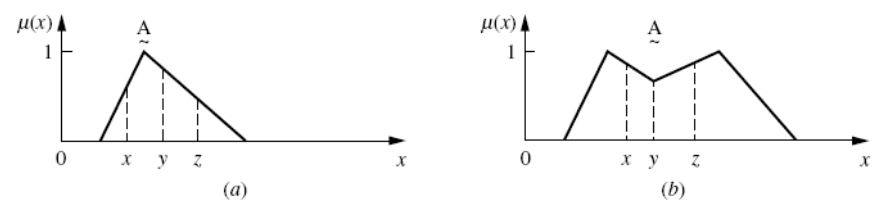
\includegraphics[width=0.7\linewidth]{img/convex}
	\caption{Eine konvexe Fuzzy-Menge (a) und eine nicht konvexe Fuzzy-Menge (b)}
	\label{fig:convex}
\end{figure}


\subsubsection{Linguistische Terme}

Um auf eine Fuzzy-Mengen innerhalb des Fuzzifizierungs-Interface oder der Entscheidungslogik zu referenzieren, werden den Fuzzy-Mengen Linguistische Terme zugeordnet. Linguistische Terme sind formal nur Bezeichner für Fuzzy-Mengen. Es ist jedoch Sinnvoll erst den Linguistische Term und anschließend die dazu passende Fuzzy-Menge zu konstruieren. Die Definition dieser Zugehörigkeit wird auch Partitionierung genannt. Es ist Aufgabe des Domain-Experten, also eine Person die das System sehr gut kennt, diese Partitionierung vorzunehmen.


\begin{defnt}
Eine Linguistischer Term ist eine umgangssprachliche Beschreibung einer Fuzzy-Menge, also \enquote{Sehr groß}$\rightarrow X \rightarrow \left[0,1\right]$
\end{defnt}


\begin{bsp} 
Eine Familie ist auf der Suche nach einer neuen Wohnung. Ein wichtiges Kriterium für die neue Wohnung sind die Anzahl der Räume. Der Linguistische Terme \enquote{angemessene Anzahl von Räumen für eine Familie mit 3 Kindern} könnte sich durch diese Fuzzy-Menge beschreiben lassen: $\mu: {1...8} \rightarrow  \left[0,1\right]$ mit folgenden Zugehörigkeitsgraden: $\mu(1) = 0,\:\mu(2) = 0.2,\:\mu(3) = 0.5, \mu(4) = 0.7,\mu(5) = 1, \mu(6) = 1, \mu(7) = 0.8
\mu(8) = 0.2$. Bei diese Fuzzy-Menge wird nur der Wertbereich $1...8$ betrachtet. Die Fuzzy-Menge sagt aus, dass 6 Räume optimal wären.
\end{bsp} 

\label{representationsformen}
\subsubsection{Repräsentationsformen}

Bisher haben wir gesehen, dass sich Fuzzy-Mengen durch die Zugehörigkeitsgrade für jedes Element $x_i$ aus $X$ definieren lassen. Wenn die $X$ nun aber einen sehr großen Wertebereich hat oder unendlich ist, lässt sich $\mu(x)$ am besten als einen geeigneten Funktionsterm ausdrücken. Wenn $X = \mathbb{R}$ dann werden oft Linguistische Terme wie \enquote{Groß} oder \enquote{Klein} verwendet. Als Interpretation von \enquote{Groß} kann z.B. eine monoton steigende Funktion mit den Parametern $a$ und $b$ gewählt werden. Wobei $a$ den Beginn des Anstiegs und $b$ den Zeitpunkt von $\mu(x) = 1$ bestimmt.

\begin{equation}
y_{a,b}(x)=\begin{cases}
0				& x \leq a \\
\frac{x-a}{b-a} & a \leq x \leq b \\
1 				& x \geq b 
\end{cases}
\end{equation}


\begin{figure}
	\centering
	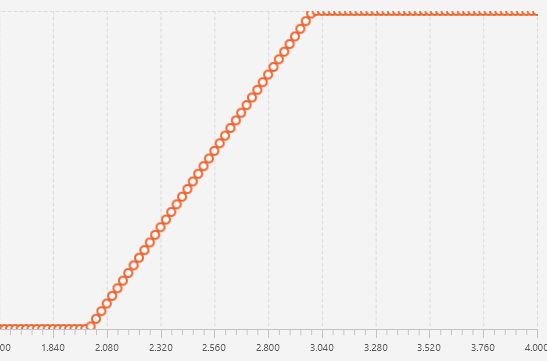
\includegraphics[width=0.5\linewidth]{img/opentriangle}
	\caption{Eine monoton steigende Funktion mit den Parametern $a=2000, b = 3000$}
	\label{fig:opentriangle}
\end{figure}

\begin{figure}
	\centering
	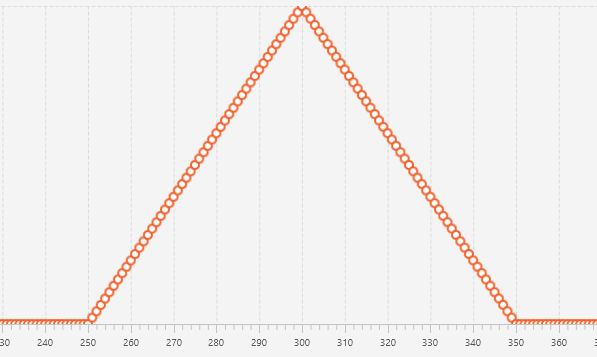
\includegraphics[width=0.5\linewidth]{img/triangle}
	\caption{Eine Dreiecksfunktion mit den Parametern $a=250, m = 300,  b = 350$}
	\label{fig:triangle}
\end{figure}

Linguistische Terme der Art \enquote{Circa 10} oder \enquote{Etwas schnell} lassen sich am besten durch symmetrische Dreiecksfunktionen ausdrücken mit den Parametern $m$ $a$ und $b$ ausrücken wobei $m$ den Mittelpunkt, $a, b$ den Start- sowie Endpunkt des Dreiecks bestimmen.

\begin{equation}
y_{a,m,b}(x)=\begin{cases}
0				& x \leq a \\
\frac{x-a}{b-a} & a \leq x \leq m  \\
\frac{b-x}{b-m} & m \leq x \leq b  \\
0 				& x \geq b \\
\end{cases}
\end{equation}

Für Linguistische Terme der Art \enquote{Zwischen 3 und 5} werden oft Trapez-Funktionen verwendet. Die Trapez-Funktion hat die Parameter $a,b,c$ und $d$. Die Parameter stellen jeweils die Kanten des Trapezes dar.

\begin{equation}
y_{a,b,c,d}(x)=\begin{cases}
\frac{x-a}{b-a} & a \leq x \leq b  \\
1 				& b \leq x \leq c \\
\frac{x-d}{c-d} & c \leq x \leq d \\
0				& x \le a \; or \; x \ge d  
\end{cases}
\end{equation}

\subsection{Fuzzy-Relationen}

Eine Fuzzy-Relation ist eine Abbildung von verschiedenen Grundmengen z. B. von zwei Variablen in einen Zugehörigkeitsgrad $\mu_{A \times B}$. In welchem Zusammenhang die Grundmengen $A$ und $B$ stehen kann entweder über eine Tabelle oder einen Fuzzy-Operator (siehe Kapitel \ref{fuzzy-operatoren}) bestimmt werden.

\label{fuzzy-operatoren}
\subsection{Fuzzy-Operatoren}

Fuzzy-Operatoren sind notwendig sobald mehrere Fuzzy-Mengen miteinander verknüpft werden sollen. Aus der klassischen Mengenlehre kennt man die Operatoren Komplement, Durchschnitt und Vereinigung. Diese wurden auch in der Originalarbeit aus dem Jahr 1965 von Zadeh wie folgt für Fuzzy-Mengen definiert.

\begin{defnt}[Komplement]
	Das Komplement bzw. die NICHT-Operation ist definiert als: 
	\begin{equation}
		(\forall x \in X) : \mu_{\not A}( x) = 1 - \mu_A(x)
	\end{equation}
	
\end{defnt}

\begin{defnt}[Durchschnitt]
	Der Durchschnitt bzw. die UND-Operation ist definiert als: 
	\begin{equation}
		(\forall x \in X) : \mu_{A \bigcap B}( x) = min(\mu_A(x),\mu_B(x))
	\end{equation}
\end{defnt}

\begin{defnt}[Vereinigung]
	Die Vereinigung bzw. die ODER-Operation ist definiert als: 
	\begin{equation}
		(\forall x \in X) : \mu_{A \bigcup B}( x) = max(\mu_A(x),\mu_B(x))
	\end{equation}	  
\end{defnt}

Es gibt jedoch die Möglichkeit diese Funktionsdefinitionen für die Operationen durch andere Funktionen zu ersetzen solange die sogenannte t-Norm für diese eingehalten wird. So hat zum Beispiel die Verwendung des Minimums den Nachteil, dass manche Werte nicht beachtet werden.

\begin{defnt}
	Eine Funktion $F: \left[0,1\right]^2 \rightarrow \left[0,1\right]$ heißt t-Norm, wenn folgende Bedingen gelten: Kommutativität, Assoziativität, Monotonie sowie die Existenz eines neutralem Elements.
	
\end{defnt}

\section{Fuzzy-Regler}

Um die Grundbegriffe der Regelungstechnik zu verstehen betrachten wir ein System, wie z.B. einen Gleichstrom Motor einer Drohne oder eine Wohnraumheizung. Der Benutzer eines solches System gibt der Regelungstechnik einen bestimmten Sollwert vor. Der Sollwert sollte Messbar seien und sich in einem bestimmten Wertebereich befinden. So könnte der Sollwert für den Drohnennmotor die Drehzahl 1500 Rounds per Minute(RPM) seien oder der Sollwert für die Heizung eine Temperatur von \SI{22.0}{\celsius}. Interessant für die Regelungstechnik ist hierbei, dass die Systeme träge sind und nicht direkt auf Änderung reagieren sowie das Vorkommen von Störgrößen, die das System beeinflussen. Ein Störgröße für die Wohnraumheizung könnte z.B. ein offenes Fenster sein das die Temperatur beeinflusst. Die Aufgabe der Regelungstechnik ist es nun das System möglichst konstant auf dem Sollwert zu halten. Dazu wird eine Stellgröße $\eta$ von der Regelungstechnik reguliert. Für den Motor könnte die Stromzufuhr und für Heizung die Ventilstellung eines Thermostats die Stellgröße darstellen. Die letztendliche Ausgangsgröße setzt sich also aus Stellgröße und Störgröße zusammen. Ein neuer Stellwert von der Regelungstechnik auf Basis der Messwerte (Eingangsgrößen) für die Ausgangsgröße $\xi$ und die zeitliche Änderung der Ausgangsgröße $\Delta\xi = \frac{d\xi}{dt}$ berechnet. Wir gehen davon aus, dass die Stellgröße einen Wert der Menge $Y$ annehmen kann und die Eingangsgrößen, oder auch Meßgrößen, $\xi_{i=1...n}$ (ebenfalls $\xi$ weil die Ausgangsgröße oft als Messgröße wiederverwendet wird) einen Wert de Menge $X_i$ annehmen kann. Es wird also eine Kontrollfunktion $\varphi: X_0...X_n \rightarrow Y$ gesucht.

\begin{figure}
	\centering
	\includegraphics[width=0.7\linewidth]{img/regelungstrecke}
	\caption[Aufbau einer Regelstrecke]{Aufbau eine Regelstrecke}
	\label{fig:regelungstrecke}
\end{figure}


\subsection{Vorteile des Fuzzy-Reglers}

Um den Vorteil eines Fuzzy-Reglers zu verstehen, sollte man sich zuerst konkretes regelungstechnisches Problem vor Augen führen. In den folgenden Kapiteln betrachten wir das Stabbalance-Problem aus Beispiel \ref{bsp:stab}. 

\begin{bsp} 
	\label{bsp:stab}
	Das Stabbalance-Problem beschreibt ein System in dem ein Stab mit der Masse $m$ am Kopfende, der Masse $M$ am Fußende und der Länge $l$ vertikal, also parallel zur Erdanziehungskraft, ausbalanciert werden soll. Das untere Ende des Stabs darf in horizontaler Achse bewegt werden. Diese Bewegung stellt unsere Stellgröße $F$ dar. Die Ausgangsgröße ist der Winkel $\Theta$ des Stabs relative zur vertikalen Achse. Also wird $\Theta$ positiv, wenn der Stab nach rechts fällt und negative wenn der Stab nach links fällt. Zusätzlich zu dem Winkel $\Theta$ wird auch die Winkelgeschwindigkeit, also die Veränderung des Winkels, $\dot{\Theta} = \frac{d\Theta}{dt}$ betrachtet. Der Wertebereich $X_1$ für den Winkel $\Theta$ definieren wir im Intervall $\left[-90,90\right]$ in der Einheit Grad und den Wertebereich $X_2$ im Intervall $\left[-45, 45\right]$ in der Einheit $Grad \cdot s^{-1}$. Die Kraft $F$ wird in der Einheit Newton im Intervall von $-10$ bis $+10$ definiert, also $Y=\left[-10, 10\right]$.
\end{bsp}

Die klassische Regelungstechnik setzt voraus, dass das zu regelnde System durch ein physikalisch-mathematisches Modell beschrieben werden kann. Das oben genannte Stabbalance-Problem lässt sich durch die folgende Differentialgleichung beschreiben (siehe Gl. \ref{eq:stabdiff}). In dieser Gleichung ist $F(t)$ so zu wählen, dass $\Theta(t)$ gegen Null konvergiert für $t \rightarrow \infty$. Der Vorteil bei diesem Problem ist, dass es ein mathematisches Modell gibt das den physikalischen Prozess des Systems annähernd gut beschreiben kann. Für viele andere Systeme gibt es jedoch kein bekanntes Modell oder dieses, in Form einer weiteren Differentialgleichung, lässt sich schwer lösen.

\label{eq:stabdiff}
\begin{equation}
(M+m)sin^2 \Theta \cdot l \cdot \ddot{\Theta} + m \cdot l \cdot \Theta \cdot cos\Theta \cdot \dot{\Theta}^2 - (m + M) \cdot g \cdot sin \Theta = -F \cdot cos \Theta
\end{equation}

Der Mensch kann das Stabbalance-Problem, mit ein wenig Übung, problemlos regulieren. Es ist also doch möglich das Stabbalance-Problem zu bewältigen ohne die Differentialgleichung zu lösen oder das physikalisch-mathematisches Modell verstanden zu haben. Die sogenannte \enquote{kognitive Analyse} versucht das Wissen bzw. das Verhalten des Menschen zu extrahieren und daraus ein Modell zu gestalten. Es wird also versucht das Verhalten des Menschen nachzubilden. Diesem alternativen Ansatz wird bei der Fuzzy-Regelung nachgegangen.

\subsection{Komponenten eines Fuzzy-Reglers}

In diesem Kapitel werden die verschiedenen Komponenten einer Fuzzy-Regelung erläutert. Ein Fuzzy-Regler besteht im allgemeinen aus einem sogenannten Fuzzifizierungs-Interface, der Wissensbasis, der Entscheidungslogik sowie dem Defuzzifizierungs-Interface. Die Komponenten und deren Zusammenhänge werden in Abbildung \ref{fig:fuzzyregler} dargestellt.

\begin{figure}
	\centering
	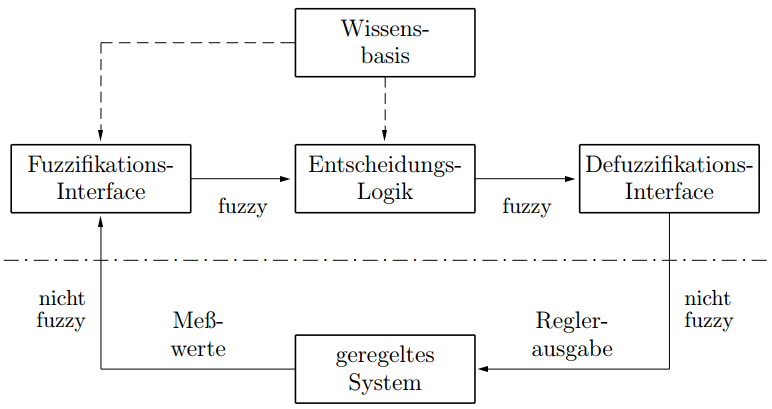
\includegraphics[width=0.7\linewidth]{img/fuzzyregler}
	\caption{Aufbau eines Fuzzy-Reglers.}
	\label{fig:fuzzyregler}
\end{figure}

\subsubsection{Wissensbasis}

Die Wissensbasis besteht aus der Regelbasis und der Datenbasis. Alle Wertebereiche für die Eingangsgrößen und Stellgrößen $X_ {1...n}, Y$ sowie die dazugehörigen linguistischen Termen und dazu assoziierten Fuzzy-Mengen gehören zu der Datenbasis. Die Regelbasis besteht aus den linguistischen Kontrollregeln.

\subsubsection{Fuzzifizierungs-Interface}

Bei der sogenannten Fuzzifizierung geht es darum die kontinuierlichen analogen Eingangswerte aus den Definitionsmenge $X_i$ in eine Menge von Zugehörigkeitsgraden zu den Fuzzy-Mengen $F(X)$ umzuwandeln. Die Menge aller Zugehorigkeitsgrade zu $F(X)$ kann so als fuzzifizierte Eingangsgröße angesehen werden. Diese Einganggrößen verändern ihren Wert stetig wenn sich die analogen Eingangswerte verändert. 

\subsubsection{Entscheidungslogik}

Die Entscheidungslogik versucht aus der bereits fuzzifizierten unscharfen Eingangsgröße eine unscharfe Ausgangsgröße oder Stellgröße abzuleiten. Dazu wird eine sogenannte Regelbasis benötigt. Die Regelbasis besteht aus eine Menge von Kontrollregeln die meist von einem Domain-Experten aufgestellt werden.

\subsubsection{Defuzzyfizierungs-Interface}

Das Defuzzyfizierungs-Interface wandelt die Stellgröße, die in Form einer Fuzzy-Menge ausgedrückt wird, in einen scharfen Wert um. Dazu werden unterschiedliche Defuzzyfizierungs-Methoden verwendet. Die Methoden werden in Kapitel \ref{defuzzy} erläutert.


\subsection{Varianten der Fuzzy-Regelung}

Es haben sich zwei Arten von Fuzzy-Reglern etabliert. Zum einen gibt es den Ansatz von Mamdani und den Ansatz Takagi und Sugeno. Die auf Takagi und Sugeno zurückgehende Methode der Fuzzy-Regelung entspricht einer Modifizierung des Ansatzes von Mamdani. Deshalb wird die Funktionsweise des Mamdani-Reglers zuerst erläutert.

Das allgemeine Entwurfsschema für einen Fuzzy-Regler ist:

\begin{enumerate} 
	\item Festlegung der Ein- und Ausgangsgrößen.
	\item Festlegung der linguistischen Variablen durch Terme samt Zugehörigkeitsfunktion.
	für die in 1. eingeführten Größen.
	\item Erstellung der Regelbasis.
	\item Festlegung der Methoden zur Fuzzyfizierung und Defuzzyfizierung.
	\item Festlegung der Inferenzmethode.
\end{enumerate}

\subsubsection{Ansatz von Mamdani}

Bei diesem Ansatz formuliert der Experte des Systems eine Liste von $k$ verschiedenen linguistischen Regeln  der Form:

\begin{equation}
	\textbf{if} \; \xi_1 \; \textbf{is} \; A_{i1} \; \textbf{and... and} \; \xi_n \; \textbf{is} \; A_{in} \; \textbf{then} \; \eta \;\textbf{is} \;B
\end{equation}

Wobei $A_{i1},...,A_{in}$ und $B$ linguistische Terme sind. Diese müssen bereits vorher vom Experten des Systems bestimmt und den entsprechenden Fuzzy-Mengen zugeordnet werden. Diesen Vorgang nennt man auch Partitionierung. Dazu werden auf der Menge der Eingangsgrößen $X_{i=1...n}$ und der Ausgangsgröße $Y$ $p$ verschiedene Fuzzy-Mengen definiert und jede dieser Fuzzy-Mengen mit einem linguistischem Term zugeordnet. Hierzu können die in Kapitel \ref{representationsformen} erläuterten Repräsentationsformen wie z.B. Dreiecksfunktionen oder Trapezfunktionen verwendet werden. Der Experte kann bei der Partitionierung entscheiden wie fein oder grob er den Wertebereich unterteilen möchte. Bei einer groben Partitionierung mit z.B. drei Fuzzy-Mengen benötigt man nicht viele Regeln und die Berechnung erfolgt schnell. Eine feinere Partitionierung mit fünf, sieben oder neun Fuzzy-Mengen liefert eine feinere Regelung. Oft werden linguistische Terme wie \enquote{Negativ groß}, \enquote{Negativ klein}, \enquote{Ungefähr Null}, \enquote{Positiv klein} und \enquote{Positiv groß} gewählt. Häufig werden die Fuzzy-Mengen so aufgeteilt, dass sie sich höchstens bis zu einem maximalen Grad von 0.5 überschneiden. Dies wird als Disjunktheitsforderung bezeichnet. Ein Beispiel für eine Partitionierung ist in Abbildung \ref{fig:partitionierung} zu sehen.

\begin{figure}
	\centering
	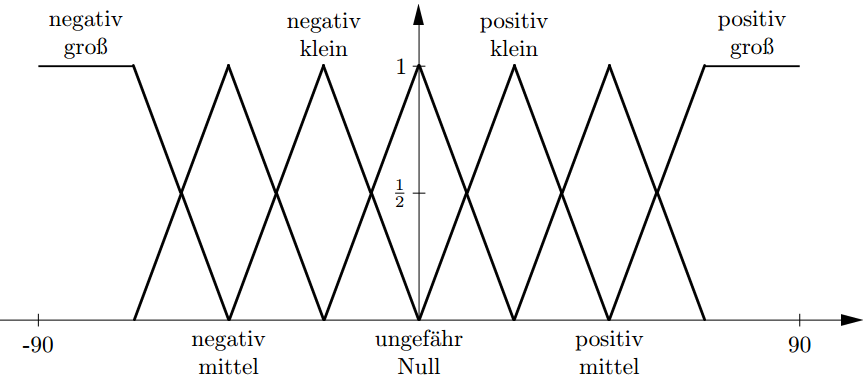
\includegraphics[width=0.7\linewidth]{img/partitionierung}
	\caption{Partiotionierung in 7 Fuzzy-Mengen. $ Y \rightarrow \left[-90,90\right]$}
	\label{fig:partitionierung}
\end{figure}


\begin{defnt}
	Disjunktheitsforderung: 
	\begin{equation}
		i \neq j \rightarrow sup_{x \in X} (min(\mu_i(x), \mu_k(x))) \leq 0.5
	\end{equation}
\end{defnt}

Jede der $1...k$ Regeln trägt nun einen Teil der Definition von $\eta = \varphi(\xi_1,..., \xi_n)$ bei. So wird jede Regel einzeln ausgewertet und dann mit der festgelegten Inferenzmethode zu der gesamt Lösung hinzugefügt.

Diese Auswertung einer Regel lässt sich in drei Schritte unterteilen:

\begin{enumerate} 
	\item Prämissenauswertung
	\item Aktivierung
	\item Aggregation
\end{enumerate}

\paragraph{Prämissenauswertung}

Für die Auswertung einer Regel wird zunächst der Akzeptanzgrad dieser Regel bestimmt. Dazu wird für jeden linguistischen Term der Prämisse der Zugehörigkeitsgrad für den kürzlich gemessene Messwert bestimmt. Also $\mu_v (x_v)$ mit $v = 1...n$. Da es in einer Regel mehrere Prämissen geben kann, die mit den Operatoren $\left[and, or\right]$ verknüpft werden können, müssen auch die Zugehörigkeitsgrade der $n$-verschiedenen Prämissenteilen durch eine geeignete Konjunktion, z.B. Minimum für $and$-Verknüpfungen, verknüpft werden (siehe Kapitel \ref{fuzzy-operatoren}).

\paragraph{Aktivierung}

Die Konklusion ergibt eine Fuzzy-Menge von Stellwerten. Um die Aktivierung der Konklusion zu bestimmen muss der linguistische Term mit dem Akzeptanzgrad der Prämisse verknüpft werden. Dazu wird die sogenannte Inferenzmethode gewählt. Die zwei meist verbreitetsten Methoden sind: 

\begin{enumerate} 
	\item MAX-MIN-Inferenz
	\item MAX-PROD-Inferenz
\end{enumerate}

\subparagraph{MAX-MIN-Inferenz}

Bei der MAX-MIN-Inferenz wird die Ausgabe Fuzzy-Menge $B$ an der Höhe des minimalen Akzeptanzgrad der Prämisse gekappt. 

\begin{equation}
	output^{R_r}_{x_1...x_n}:  y \mapsto min(\mu_{1,r}(x_1), ..., \mu_{n,r}(x_n), \mu_r(y))
\end{equation}

\subparagraph{MAX-PROD-Inferenz}

Bei der MAX-PROD-Inferenz wird die Ausgabe Fuzzy-Menge $B$ mit der Summe der Akzeptanzgrade multipliziert. Bei der SUM-PROD-Inferenz entstehen u.U. Fuzzy-Mengen mit einem Zugehörigkeitsgrad größer 1. Solche Fuzzy-Mengen nennt man nicht normierte Fuzzy-Mengen.

\begin{equation}
output^{R_r}_{x_1...x_n}:  y \mapsto \sum_{i = 1}^{n} \mu_{i,r}(x_i) \cdot \mu_r(y)
\end{equation}

Für beide Inferenzmethoden gilt, dass in dem Fall das der Akzeptanzgrad 1 ist d.h. erfüllen die Messwerte die Prämisse der Regel vollständig, liefert die Regel gerade ihre Konklusions-Fuzzy-Menge als Ausgabe. Falls der Akzeptanzgrad 0 ist, wird eine Fuzzy-Menge geliefert, die immer 0 ist.

\paragraph{Aggregation}

Die Ausgabe aktivierten Fuzzy-Mengen $B_{1...k}$ werden mithilfe der Maximumbildung zusammengefügt. Diese eine Ausgangs Fuzzy-Menge $	output_{x_1,..., x_n}$ wird dann an das Defuzzifizierungs-Interface übergeben und mit der gewählten Defuzzifizierungs-Methoden (siehe Kapitel \ref{defuzzy}) in einen scharfen Wert umgewandelt.

\begin{equation}
	output_{x_1,..., x_n}: y \mapsto \max_{r \in (1,...,k)}(output^{R_r}_{x_1...x_n})
\end{equation}

\subsubsection{Ansatz von Takagi und Sugeno}

Die auf Takagi und Sugeno zurückgehende Methode der Fuzzy-Regelung entspricht einer Modifizierung des Ansatzes von Mamdani. In der Konklusion der Regeln stehen im Gegensatz zu Fuzzy-Reglern nach Mamdani keine Fuzzy-Mengen sondern Funktionen der Eingangsgrößen. Die Funktionswerte werden mit den Akzeptanzgraden  der Regeln gewichtet. Das Ergebnis ist die scharfe Stellgröße. Es ist also keine Defuzzyfizierung notwendig. Die Regeln des Takagi und Sugeno Reglers haben die Form:

\begin{equation}
\textbf{if} \; \xi_1 \; \textbf{is} \; A_{i1} \; \textbf{and... and} \; \xi_n \; \textbf{is} \; A_{in} \; \textbf{then} \; \eta \; = f_r(\xi_1,..., \xi_n)
\end{equation}

Wobei $f_r$ eine Abbildung von $X_1 \times, \dotsc, \times X_n \mapsto Y (r = 1 ,\dotsc, k)$ ist. Oft hat $f_r$ die Form: $f_r(x_1,..., x_n) = p_0^r + p_1^r \cdot x_1 + \dotsb + p_n^r * x_n$. Die Parameter der Regel $p_0^r, \dotsc, p_n^r$ liegen in einer Tabelle ab. Die Entscheidungslogik wertet für jede Regel den Akzeptanzgrad der Prämisse $a_r$ aus. Dazu wird nur der Schritt Prämissenauswertung des Madmani-Ansatz gebraucht. Anschließend wird die mit dem Akzeptanzgrad der Prämissen gewichtete Summe der Ausgabewerte der einzelnen Regeln als Stellwert verwendet.
\begin{equation}
\eta = \frac{\sum_{i=1}^{r} a_r \cdot f_r(x1, \dotsc, x_n)}{\sum_{i=1}^{r} a_r}
\end{equation}

\begin{bsp}
	\label{bsp:takagi}
	Ein nichtlinearer statischer Regler, dessen Übertragungskennlinie in der Nähe der Regelabweichung eine geringere Verstärkung aufweist als im übrigen Bereich implementiert als Takagi und Sugeno Regler. Dazu definieren wir den die Eingangsgröße $\xi_1 = e \text{ mit } Y \mapsto \left[-1,+1\right]$. Die Eingangsgröße $e$ stellt eine Regelabweichung (Sollwert $ - $ Eingangswert) dar. Es werden die drei Regeln festgelegt:
	
	\begin{gather*}
	\textbf{Regel 1: } \; \textbf{if} \; e \; \textbf{is} \; \text{kleiner null} \; \textbf{then} \; \eta \; = 2,5 \cdot e  \\ 
	\textbf{Regel 2: } \; \textbf{if} \; e \; \textbf{is} \; \text{ungefähr null} \; \textbf{then} \; \eta \; = 0,4 \cdot e   \\ 
	\textbf{Regel 3: } \; \textbf{if} \; e \; \textbf{is} \; \text{größer null} \; \textbf{then} \; \eta \; = 2,5 \cdot e
	\end{gather*}
	
	Wenn wir nun den Eingangswert $e=-0,8$ betrachten erhalten wir folgende Zugehörigkeitsgrade für die linguistischen Terme und somit auch die Aktzeptanzgrade für die Regeln 1-3, da jede Regel nur einen linguistischen Term benutzt:
	\begin{gather*}
		\mu_{\text{kleiner null}} (e) = 0,8 ,\; \mu_{\text{ungefähr null}} (e) = 0,2 ,\; \mu_{\text{größer null}}(e) = 0 \\
		a_{r1} (e) = 0,8 ,\; a_{r2} (e) = 0,2 ,\; a_{r3}(e) = 0
	\end{gather*}
	
	Da die dritte Regel einen Aktzeptanzgrade von $0$ hat, wird diese nicht mehr in die Lösung mit einbezogen.
	
	\begin{gather*}
		 \eta = \frac{0,8 \cdot 2,5 \cdot -0,8 + 0,2 \cdot 0,4 \cdot -0,8}{0,8 + 0,2} = -1,664
	\end{gather*}

	\begin{figure}
		\centering
		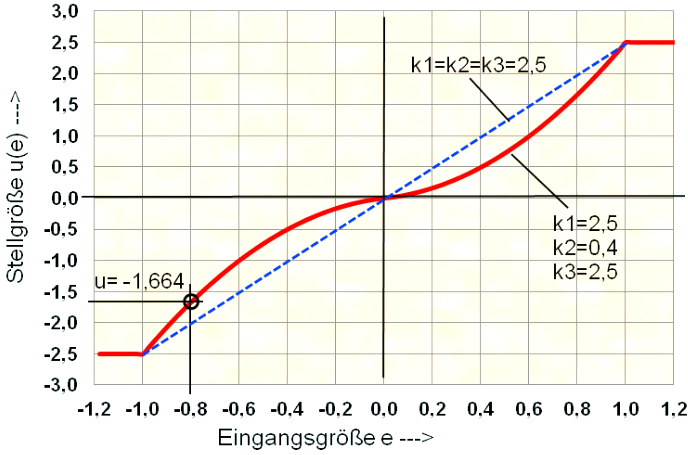
\includegraphics[width=0.7\linewidth]{img/Takagi}
		\caption{Übertragungskennlinie des Takagi-Sgeno-Reglers aus Beispiel \ref{bsp:takagi} (hier $k1, ..., k3$ für $p^1, ..., p^3$ )}
		\label{fig:takagi}
	\end{figure}

	Die daraus resultierende Kennlinie ist in Abbildung \ref{fig:takagi} zu erkennen. Wenn die Parameter $p^1, ..., p^3$ geändert werden sollten, ändert sich auch diese Kennlinie.
\end{bsp}

\subsubsection{Vorteile}

Da nun die beiden Ansätze für Fuzzy-Controller vorgestellt wurde, wollen wir in einer Liste aufführen welche Vorteile der jeweilige Regler hat.

\paragraph{Vorteile der Mamdani Methode}

\begin{itemize}
	\item Dem Menschen fällt es leicht die Wissensbasis aufzustellen.
	\item Mamdani Regler haben einen hohen Bekanntheitsgrad.
	\item Am häufigsten eingesetzt.
	\item Sehr intuitiv zu verstehen.
\end{itemize}

\paragraph{Vorteile der Takagi und Sugeno Methode}

\begin{itemize}
	\item Arbeitet sehr effizient (keine Defuzzifizierungs Methode notwendig).
	\item Kann auch in Kombination mit anderen linearen Reglern eingesetzt werden.
	\item Lässt sich gut optimieren.
	\item Gut geeignet für mathematische Analysen
\end{itemize}

\label{defuzzy}
\subsection{Defuzzifizierungs-Methoden}

Das Defuzzifizierungs-Interface erhält aus der Entscheidungslogik eine Fuzzy-Menge und soll daraus nun einen scharfen Stellwert ermitteln. Diesen Vorgang nennt man Defuzzifizierung. Es gibt verschiedene Defuzzifizierung-Methoden die diesen Prozess definieren. Die wichtigsten werden nun vorgestellt. Um die Wirkung der Defuzzifizierungs-Methoden auf die Stellgröße zu visualisieren betrachten wir ein Beispiel. Für jede Methode wird  ein Plot der Stellgröße im Verlauf der Simulation des Beispiels gezeigt.

\begin{bsp}
	Ein durch eine Fuzzy-Regelung gesteuertes Auto soll einem anderen Auto folgen und einen angemessenen Abstand halten. Die Fuzzy-Regelung betrachtet dazu die Messgrößen Geschwindigkeit und Abstand und gibt die Stellgröße der Beschleunigungskraft $y \rightarrow \left[-8000, +4000\right]$ in der Einheit Newton. Diese Kraft stellt die Bremskraft sowie die Beschleunigungskraft dar. In der Simulation lassen wir das vordere Auto erst für 15 Sekunden mit voller Beschleunigung davon fahren und initiieren danach eine Vollbremsung. Das hintere Auto versucht den Abstand durch eine Fuzzy-Regelung zu kontrollieren.
\end{bsp}

\subsubsection{Maximum-Kriterium-Methode}

Die Maximum-Kriterium-Methode ist die einfachste Defuzzifizierungs-Methoden. Sie wählt einen beliebigen Wert aus $y \in Y$ aus für den die Zugehörigkeitsfunktion der Ausgangs-Fuzzy-Menge $output_{x_1,..., x_n}$ ihren maximalen Zugehörigkeitsgrad hat. Da hier nicht deterministisch gewählt wird, kann dies unter Umständen zu einem sprunghaften Stellverhalten führen. Dies geschieht genau dann, wenn es mehr als einen Wert $y \in Y$ mit $y = \max_{y \in Y}(output_{x_1,..., x_n}(y))$ gibt. Dies kann aber auch von Vorteil sein, wenn die Stellgröße keinen reellen Wert sondern z.B. eine Stellaktion darstellt. Anderenfalls führt diese Defuzzifizierungs-Methoden zu einem sprunghaften Regelverhalten. Dieses Verhalten ist gut in Abbildung \ref{fig:max} zu erkennen. 

\begin{equation}
	output_{x_1,..., x_n}(\eta) \geq output_{x_1,..., x_n}(y) \forall y \in Y
\end{equation}

\begin{figure}
	\centering
	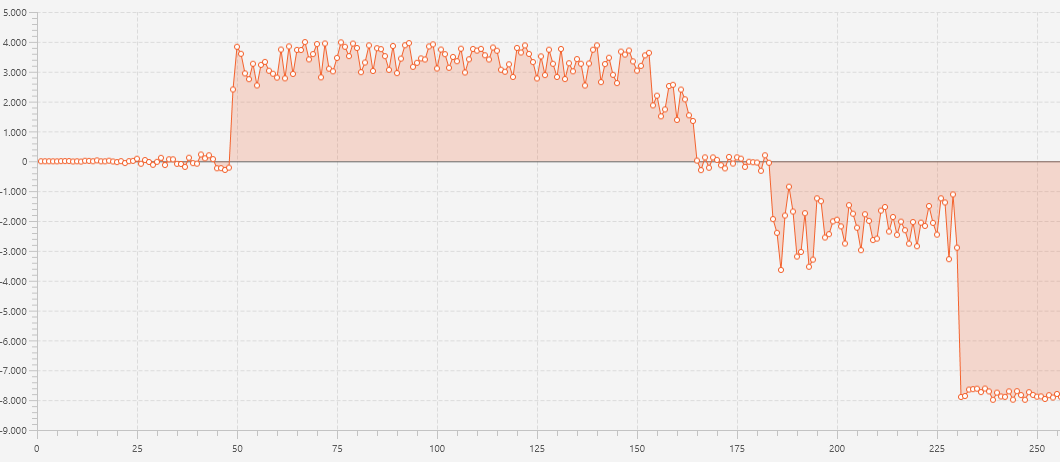
\includegraphics[width=0.8\linewidth]{img/defuzzy/max3}
	\caption{Verlauf der Stellgröße $\eta$ in der Beispielsimulation unter Verwendung der Maximum-Kriterium-Methode}
	\label{fig:max}
\end{figure}

\subsubsection{Mean-of-Maxima-Methode}

Die Mean-of-Maxima-Methode (MOM) wählt einen scharfen Stellwert indem sie den Mittelwert über die Menge $\max(output_{x_1,..., x_n})$ berechnet. Bei dieser Methode kann es vorkommen, dass $\eta \notin  \max(output_{x_1,..., x_n})$ gilt. Dies tritt bei nicht konvexen Ausgabe Fuzzy-Mengen auf und kann zu unvorhergesehen Folgen führe (siehe Beispiel \ref{fuzzyfail}). Die MOM-Methode führt außerdem, wenn symmetrischen Dreiecksfunktionen für die Partitionierung von $Y$ verwendet wurden, zu einem, unstetigen Verlauf der Stellgröße. Grund hierfür ist, dass eine Regel stets den Ausgang dominiert. Dies kann in physikalischen System eine starke Belastung für die Stellvorrichtung sein. Das sprunghafte Verhalten ist gut in Abbildung \ref{fig:mom} zu erkennen. 
 

\begin{equation}
\eta = \frac{1}{ | \max(output_{x_1,..., x_n)} | } \cdot \sum_{y\in \max(output_{x_1,..., x_n})} y
\end{equation}

\begin{figure}
	\centering
	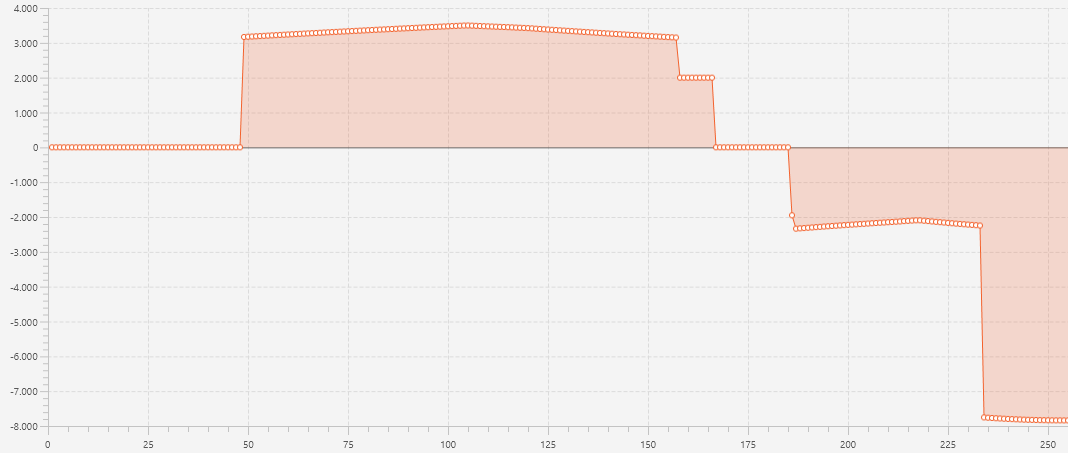
\includegraphics[width=0.8\linewidth]{img/defuzzy/mom3}
	\caption{Verlauf der Stellgröße $\eta$ in der Beispielsimulation unter Verwendung der Mean-of-Maxima-Methode}
	\label{fig:mom}
\end{figure}

\subsubsection{Center-of-Gravity-Methode}

Die Center-of-Gravity-Methode (COG) wählt einen scharfen Stellwert indem sie den Flächeninhalt zwischen der Funktion $output_{x_1,..., x_n)}$ und der X-Achse betrachtet und daraus den Schwerpunkt berechnet. Der Stellwert ist dann die X-Koordinate dieses Schwerpunktes. Vorteil bei dieser Methode ist, dass fast immer ein stetiger Regelverlauf generiert wird. Grund hierfür ist, dass auch alle Regeln mit ihrem Akzeptanzgrad berücksichtigt werden. Erst wenn die Messgrößen jetzt so stark springe, dass der Akzeptanzgrad einer Prämisse innerhalb eines Berechnungsschrittes von einem relative hohen Wert auf 0 sinkt, springt auch der Stellwert der COG-Methode.

\begin{equation}
\eta = \frac{1}{\int_{y \in Y} output_{x_1,..., x_n}(y) dy} \cdot \int_{y \in Y} y \cdot output_{x_1,..., x_n}(y)dy
\end{equation}

\begin{figure}
	\centering
	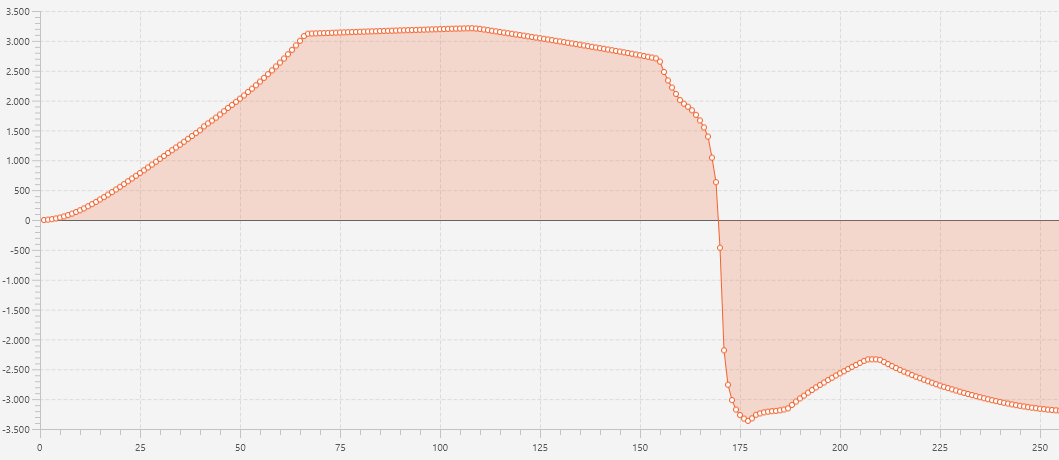
\includegraphics[width=0.8\linewidth]{img/defuzzy/center1}
	\caption{Verlauf der Stellgröße $\eta$ in der Beispielsimulation unter Verwendung der Center-of-Gravity-Methode}
	\label{fig:cog}
\end{figure}

\begin{bsp}
	Die Defuzzifizierung der in Abbildung \ref{fig:defuzzy} dargestellten Fuzzy-Menge gibt als Stellgröße $F = \left[4,6\right]$ für die Maximum-Kriterium-Methode, $F = 5$ für die MOM-Methode und $F \approx 3,95$ für die COG-Methode.
\end{bsp}

\begin{figure}
	\centering
	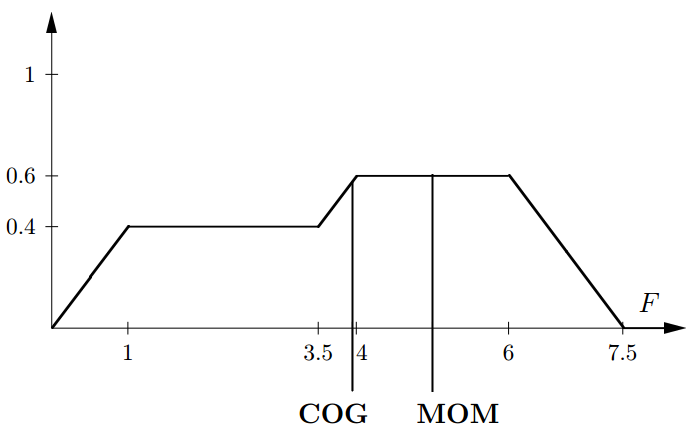
\includegraphics[width=0.7\linewidth]{img/defuzzy/defuzzy}
	\caption{Stellwerte der verschiedenen Defuzzifikationsmethoden für eine Fuzzy-Menge.}
	\label{fig:defuzzy}
\end{figure}

\subsubsection{Auswahlkriterien}

Neben den drei vorgestellten Defuzzifizierungs-Methoden gibt es noch diverse Erweiterungen bzw. Varianten sowie weitere Methoden zur Defuzzyfizierung. Nun kommt die Frage auf, welche dieser Methoden nun die Beste sei und die Antwort auf diese Frage ist, dass es sehr Kontext- bzw. Problemabhängig ist. Wir betrachten nun fünf Kriterien die bei der Auswahl der richtigen Defuzzifizierungs-Methoden helfen sollen \cite{175683}.

\begin{enumerate} 
	\item Stetigkeit
	\item Eindeutigkeit
	\item Plausibilität
	\item Rechenaufwand
	\item Gewichtung
\end{enumerate}

\paragraph{Stetigkeit}

Wenn der Stellwert große Sprünge hat, könnte dies negative Auswirkung auf die Regelstrecke sowie das Stellglied haben. Trotzdem könnte es auch Systeme geben für die Stetigkeit keine Rolle spielen oder ein sprunghaftes Verhalten sogar besser ist wie z.B ein System mit Stellaktionen. Ein stetige Methode verändert bei geringer Änderung der Messgrößen nie viel an der Stellgröße.

\paragraph{Eindeutigkeit}

Falls die Methode für einen Eingang $\xi_{1...n}$ immer den gleichen Ausgang $\eta$ erzeugt, ist diese Eindeutig. Dieses Kriterium könnte z.B. bei sicherheitsrelevanten System eine harte Anforderung sein.

\paragraph{Plausibilität}

Die Stellwert $\eta$ sollte einen möglichst hohen Zugehörigkeitsgrad $output_{x_1,..., x_n}(\eta)$ haben und in einer Region liegen die von einer Regel bedeckt wird. Dazu ein negativ Beispiel:

\begin{bsp}
	\label{bsp:fuzzy}
	Es wird ein Fuzzy-Regler betrachtet der ein selbst fahrendes Automobil steuern soll. Taucht nun ein Hindernis direkt vor dem Auto auf könnte die Abbildung \ref{fig:fuzzyfail} eine Ausgabe Fuzzy-Menge darstellen. Der linke Teil der Fuzzy-Menge könnte dem linguistischen Term \enquote{Lenke nach links}, der Rechte \enquote{Lenke nach rechts} entsprechen.  $Y \rightarrow \left[-180,180\right]$ in der Einheit Grad (absolute Lenkradposition). Sowohl die MOM- als auch die COG-Methode liefern jedoch als Stellwert $\eta = 0 \; Grad$ was bedeutet, dass das Auto dem Hindernis nicht ausweichen wird. Die Plausibilität ist nicht vorhanden.
\end{bsp}

\begin{figure}
	\centering
	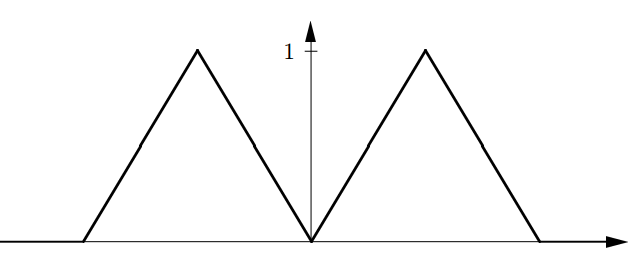
\includegraphics[width=0.7\linewidth]{img/fuzzyfail}
	\caption{AusgabeFuzzy-Menge zum Beispiel \ref{bsp:fuzzy} bei einem Hindernis gerade vor dem Auto.}
	\label{fig:fuzzyfail}
\end{figure}

\paragraph{Rechenaufwand}

Auf manchen Plattformen ist sicherlich auch relevant wie rechenintensiv die Methode sein darf. Zum Beispiel wird ein Mikrokontroller in einem Echtzeitsystem nicht die Zeit aufbringen können für jeden Regelungsschritt eine komplette Integration über den Wertebereich der Ausgangsgröße zu berechnen.

\paragraph{Gewichtung}

Gehen alle Teillösungen mit der gleichen Gewichtung in die Gesamtlösung mit ein oder wird der Akzeptanzgrad jeweils mit bedacht. Dieses Kriterium hat auch Auswirkungen auf die Stetigkeit und den Rechenaufwand. Kann aber auch wichtig sein wenn alle Regeln immer in die Lösung mit eingebracht werden sollen.

\begin{table}

\caption{Bewertung der Defuzzifizierungs-Methoden}
\begin{tabular}{|c|c|c|c|c|c|}
	\hline 
	& Stetigkeit & Eindeutigkeit & Plausibilität & Rechenauwand & Gewichtung \\ 
	\hline 
	Max-Kriterum 	& nein & nein 	& ja & sehr niedrig & nein \\ 
	\hline 
	MOM 			& nein & ja 	& nein & niedrig & nein \\ 
	\hline 
	COG 			& ja & ja 		&  nein	& hoch  &  ja \\ 
	\hline 
		
\end{tabular} 
\end{table}

% ----------------------------------------------------------------------------------------------------------

% Literatur
\nocite{*}
\bibliography{lib}
\bibliographystyle{alpha}

% ----------------------------------------------------------------------------------------------------------

\end{document}